\chapter{String Processing}

In addition to its groundbreaking expression evaluation, Unicon inherits
other compelling features from Icon that reduce the effort required to
write complex programs. Icon's ancestor is
\index{SNOBOL4}SNOBOL4, the grandfather of all string processing
languages, and from it come some of the most flexible and readable
built-in string processing facilities found in any language. In this
chapter you will learn

\begin{itemize}
\item How to manipulate strings and sets of characters
\item Icon's string scanning \index{control
structure}control structure
\item How to write custom \index{pattern matching}pattern matching
primitives, with \index{backtracking}backtracking
\end{itemize}
Techniques for matching regular expressions and context free grammars

\section{String Indexes}

You have already seen string literals delimited by double quotes, and
the most common operators that work on strings: the size of a string is
given by the unary \texttt{*} operator, substrings can be picked out
with indexes, and two strings can be concatenated with the
\texttt{{\textbar}{\textbar}} operator. Now it is time to present a
deeper understanding of the meaning of indexes as they are used with
strings and lists.

\index{string!indexes 1 based}Indexes in a string refer to the positions
between characters. The positions are numbered starting from 1. The
index 0 refers to the position after the last character in the string,
and negative indices count from the right side of the string:


\begin{center}
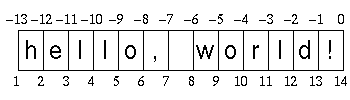
\includegraphics[width=3.6075in,height=1.0417in]{ub-img/ub-img7.png}
\end{center}
\vspace{-0.25cm}{\sffamily\bfseries Figure 3-1:}
{\sffamily Positive and Negative String Indices}

\bigskip

The expression \index{slice!string s[i:j]}\texttt{s[i:j]} refers to the
\index{substring}substring of \texttt{s} that lies between positions
\texttt{i} and \texttt{j}. If either \texttt{i} or j is not a valid
index into \texttt{s}, the expression fails. The expression
\texttt{s[k]} is short for \texttt{s[k:k+1]} and refers to a single
\index{character}character at position \texttt{k}. The expression
\texttt{s[k+:n]} is the substring of length \texttt{n} starting at
position \texttt{k}. If \texttt{s} is the string
\texttt{"hello, world!"} then the
expressions

\iconcode{
s[7] := " puny " \\
s[13:18] := "earthlings"
}

\noindent
change \texttt{s} into \texttt{"hello, puny
earthlings!"}, illustrating the ease with which
insertions and substitutions are made. The first assignment changes the
string to \texttt{"hello, puny world!"},
replacing a single character with six characters and thereby increasing
its length. The second assignment operates on the modified string,
replacing \texttt{"world"} with
\texttt{"earthlings"}.

Strings are values, just like numbers; if you copy a string and then
work on the copy, the original will be left unchanged:

\iconcode{
s := "string1" \\
new\_s := s \\
new\_s[7] := "2"
}

Now the value of \texttt{new\_s} is
"string2" but \texttt{s} is left unchanged.

As mentioned in Chapter 1, strings can be compared with string
\index{comparison operator!string}comparison operators such as
\texttt{==}.

\iconcode{
if line[1] == "\#" then ...}

If you find you are writing many such tests, the string processing you
are doing may be more cleanly handled using the string scanning
facilities, described below. But first, here is some more detail on the
character set data type, which is used in many of the string scanning
functions.

\section{Character Sets}

A cset is a set of characters. It has the usual properties of sets:
order is not significant, and a character can only occur once in a
cset. A \index{cset literal}cset literal is represented with single
quotes:

\iconcode{
c := 'aeiou'}

Since characters can only occur once in a cset, duplicates in a cset
literal are ignored; for example,
\texttt{'aaiiee'} is equivalent to
\texttt{'aie'}. Strings can be
converted to csets and vice versa. Since csets do not contain
duplicates, when a string is converted to a cset, all the duplicates
are removed.

Therefore to see if a string is composed of all the vowels and no
consonants:

\iconcode{
if cset(s) == 'aeiou' then ...}

Or, to find the number of distinct characters in a string:

\iconcode{
n := *cset(s)}

The \texttt{!} operator generates the members of a cset in sorted order;
this is also useful in some situations.

\section{Character Escapes}

Both strings and csets rely on the backslash as an escape character
within string literals. A backslash followed by an \index{escape
codes}\textit{escape code} of one or more characters specifies a
non-printable or control character. Escape codes may be specified by a
numeric value given in hex or octal format - for example,
\texttt{"{\textbackslash}x41"}.
Alternatively, any control character may be specified with an escape
code consisting of the caret (\texttt{\^{}}) followed by the alphabetic
letter of the control character. A cset containing control-C,
control-D, and control-Z could be specified as
\texttt{'{\textbackslash}\^{}c{\textbackslash}\^{}d{\textbackslash}\^{}z'}.
For the most common character escapes, a single-letter code is defined,
such as \texttt{"{\textbackslash}t"} for
the tab character, or
\texttt{"{\textbackslash}n"} for the
newline. For all other characters, the character following the
backslash is the character; this is how quotes or backslashes are
included in literals. The escape codes are summarized in Table 3-1.

\medskip
% \pagebreak

\begin{center}
{\sffamily\bfseries
Table 3-1

Escape Codes and Characters 
}
\end{center}

\begin{center}
\begin{supertabular}{|m{0.38in}|m{0.8in}|m{0.4in}|m{0.855in}|m{0.38in}|m{1.14in}|m{0.38in}|m{0.68in}|}
\hline
\sffamily\bfseries Code &
\sffamily\bfseries Character &
\sffamily\bfseries Code &
\sffamily\bfseries Character &
\sffamily\bfseries Code &
\sffamily\bfseries Character &
\sffamily\bfseries Code &
\sffamily\bfseries Character\\\hline
\ \ {\textbackslash}b &
backspace &
\ \ {\textbackslash}d &
delete &
\ \ {\textbackslash}e &
escape &
\ \ {\textbackslash}f &
form feed\\\hline
\ \ {\textbackslash}l &
line feed &
\ \ {\textbackslash}n &
newline &
\ \ {\textbackslash}r &
carriage return &
\ \ {\textbackslash}t &
tab\\\hline
\ \ {\textbackslash}v &
vertical tab &
\ {\textbackslash}' &
quote &
\ \ {\textbackslash}" &
double quote &
\ \ {\textbackslash}{\textbackslash} &
backslash\\\hline
\ {\textbackslash}\textit{ooo} &
octal &
{\textbackslash}x\textit{hh} &
hexadecimal  &
\ {\textbackslash}\^{}\textit{x} &
Control-\textit{x} &
~
 &
~
\\\hline
\end{supertabular}
\end{center}

\section{String Scanning}

Icon's string analysis facility is called
\index{string!scanning}\textit{string scanning}. A
\index{scanning!environment}scanning environment consists of a string
\index{subject string}\index{string!subject}\textit{subject} and an
integer \index{position,
string}\index{string!position}\textit{position} within the subject at
which scanning is to be performed. These values are held by the keyword
variables \texttt{\&subject} and \texttt{\&pos}. Scanning environments
are created by an expression of the form

\iconcode{
\textit{s} ? \textit{expr}}

The binary \texttt{?} operator sets the subject to its left argument and
initializes the position to 1; then it executes the expression on the
right side.

The expression usually has \index{matching functions}\textit{matching
functions} in it. Matching functions change the position, and return
the substring between the old and new positions. For example:
\texttt{move(j)}\texttt{ }moves the position \texttt{j} places to the
right and returns the substring between the old and new position. This
string will have exactly \texttt{j} characters in it. When the position
cannot move as directed, for example because there are less than
\texttt{j} characters to the right, \index{move(i)}\texttt{move()}
fails. Here is a simple example:

\iconcode{
text ? \{ \\
\>   while move(1) do \\
\>   \ \ \ write(move(1)) \\
\>   \}
}

This code writes out every other character of the string in variable
\texttt{text}.

Another function is \index{tab(i)}\texttt{tab(i)}, which sets the
position \texttt{\&pos} to its argument and returns the substring that
it passed over. So the expression \texttt{tab(0)} will return the
substring from the current position to the end of the string, and set
the position to the end of the string.

String scanning functions examine a string and generate the interesting
positions in it. We have already seen \index{find()}\texttt{find()},
which looks for substrings. In addition to the other parameters that
define what the function looks for, these string functions end with
three optional parameters: a string to examine and two integers. These
functions \index{default!scanning parameters}default their string
parameter to \texttt{\&subject}, the string being scanned. The two
integer positions specify where in the string the processing will be
performed; they default to 1 and 0 (the entire string), or
\texttt{\&pos} and 0 if the string defaulted to use \texttt{\&subject}.
Here is a \index{generator}generator that produces the words from the
input:

\iconcode{
procedure getword() \\
local wchar, line \\
\>   wchar := \&letters ++ \&digits ++
'{\textbackslash}'-' \\
\>   while line := read() do \\
\>   \ \ \ line ? while tab(upto(wchar)) do \{ \\
\>   \ \ \ \ \ \ word := tab(many(wchar)) \\
\>   \ \ \ \ \ \ suspend word \\
\>   \ \ \ \ \ \ \} \\
end
}

Variable \texttt{wchar}\texttt{ }is a cset of characters that are
allowed in words, including apostrophe (which is escaped) and hyphen
characters. \index{upto(c)}\texttt{upto(c)} returns the next position
at which a character from the cset \texttt{c} occurs. The
\index{many(c)}\texttt{many(c)} function returns the position after a
sequence of characters from \texttt{c}, if one or more of them occur at
the current position. The expression \texttt{tab(upto(wchar))} advances
the position to a character from \texttt{wchar}; then
\texttt{tab(many(wchar))} moves the position to the end of the word and
returns the word that is found. This is a generator, so when it is
resumed, it takes up execution from where it left off and continues to
look for words (reading the input as necessary).

Notice the first line: the cset \texttt{wchar} is the set union of the
upper- and lowercase letters (the value of the keyword
\texttt{\&letters}) and the digits (the keyword \texttt{\&digits}).
This cset union is performed each time \texttt{getword()} is called,
which is inefficient. Instead, the procedure ought to calculate the
value and store it for all future calls to \texttt{getword()}.

To do this, you declare the variable to be static, causing its value to
persist across calls to the procedure. Normal local variables are
initialized to the null value each time a procedure is entered. To do
this, add these two lines to the beginning of the procedure:

\iconcode{
static wchar \\
initial wchar := \&letters ++ \&digits ++
'{\textbackslash}'-'
}

The \index{match(s)}\texttt{match(s)} function takes a string argument
and succeeds if \texttt{s} is found at the current position in the
subject. If it succeeds, it produces the position at the end of the
matched substring. This expression

\iconcode{
if tab(match("-")) then sign := -1 else sign
:= 1}

\noindent
looks to see if there is a minus sign at the current position; if one is
found, \texttt{\&pos} is moved past it and the variable \texttt{sign}
is assigned a -1; otherwise, it gets a 1. The expression
\texttt{tab(match(s))} occurs quite often in string scanning, so it is
given a shortcut: \texttt{=s} does the same thing.

The last two string scanning functions to round out
Icon's built-in repertoire are
\index{any(c)}\texttt{any(c)} and \index{bal()}\texttt{bal(c1,c2,c3)}.
\texttt{any(c)} is similar to \texttt{many()}, but only tests a single
character being scanned to see if it is in cset \texttt{c}. The
\texttt{bal()} function produces positions at which a character in
\texttt{c1} occurs, similar to \texttt{upto()}, with the added
stipulation that the string up to those positions is \textit{balanced}
with respect to characters in \texttt{c2} and \texttt{c3}. A string is
balanced if it has the same number of characters from \texttt{c2} as
from \texttt{c3} and there are at no point more \texttt{c3} characters
present than \texttt{c2} characters. The \texttt{c1} argument defaults
to \texttt{\&cset}. Since \texttt{c2} and \texttt{c3} default to
\texttt{'('} and
\texttt{')'}, \texttt{bal()} defaults
to find balanced parentheses.

The restriction that \texttt{bal()} only returns positions at which a
character in \texttt{c1} occurs is a bit strange. Consider what you
would need to do in order to write an expression that tells whether a
string \texttt{s} is balanced or not.

You might want to write it as \texttt{s ? (bal() = *s+1)} but
\texttt{bal()} will never return that position. Concatenating an extra
character solves this problem:

\iconcode{
procedure isbalanced(s) \\
\>   return (s {\textbar}{\textbar} " ") ?
(bal() = *s+1) \\
end
}

If string \texttt{s} is very large, this solution is not cheap, since it
creates a new copy of string \texttt{s}. You might write a version of
\texttt{isbalanced()} that doesn't use the
\texttt{bal()} function, and see if you can make it run faster than
this version. An example later in this chapter shows how to use
\texttt{bal()} in a more elegant manner.

\subsection{File Completion}

Consider the following gem, attributed to Jerry \index{Nowlin,
Jerry}Nowlin and Bob \index{Alexander, Bob}Alexander. Suppose you want
to obtain the full name of a file, given only the first few letters of
a filename and a list of complete \index{filename completion}filenames.
The following one line procedure does the trick:

\iconcode{
procedure complete(prefix, filenames) \\
\>   suspend match(prefix, p := !filenames) \& p \\
end
}

This procedure works fine for lists with just a few members and also for
cases where \texttt{prefix} is fairly large.

\subsection{Backtracking}

\index{backtracking}The matching functions we have seen so far,
(\texttt{tab()} and \texttt{move()}), are actually
\index{generator}generators. That is, even though they only produce one
value, they suspend instead of returning. If expression evaluation ever
resumes one of these functions, they restore the old value of
\texttt{\&pos}. This makes it easy to try alternative matches starting
from the same position in the string:

\iconcode{
s ? (="0x" \& tab(many(\&digits ++
'abcdefABCDEF'))) {\textbar} \\
\>   tab(many(\&digits))
}

This expression will match either a hexadecimal string in the format
used by C or a decimal integer. Suppose \texttt{s} contains the string
\texttt{"0xy"}. The first part of the
expression succeeds and matches the
\texttt{"0x"}; but then the expression
\texttt{tab(many(\&digits ++
'abcdef'))} fails; this causes Unicon
to resume the first \texttt{tab()}, which resets the position to the
beginning of the string and fails. Unicon then evaluates the expression
\texttt{tab(many(\&digits))} which succeeds (matching the string
\texttt{"0"}); therefore the entire
expression succeeds and leaves \texttt{\&pos} at 2.

{\sffamily\bfseries
Warning}

{\sffamily
Be careful when using tab() or move() in a surrounding expression that
can fail! The fact that tab() and move() reset \&pos upon expression
failure causes confusion and bugs when it happens accidentally.}

\subsection{Concordance Example}

Listing 3-1 illustrates the above concepts and introduces a few more.
Here is a program to read a file, and generate a
\index{concordance}concordance that prints each word followed by a list
of the lines on which it occurs. Short words like
\texttt{"the"} aren't
interesting, so the program only counts words longer than three
characters. 

\bigskip

{\sffamily\bfseries Listing 3-1}
{\sffamily\bfseries A simple concordance program}

\iconcode{
procedure main(args) \\
\>   (*args = 1) {\textbar} stop("Need a
file!") \\
\>   f := open(args[1]) {\textbar}
stop("Couldn't open ",
args[1]) \\
\>   wordlist := table() \\
\>   lineno := 0 \\
\ \\
\>   while line := map(read(f)) do \{ \\
\>   \ \ \ lineno +:= 1 \\
\>   \ \ \ every word := getword(line) do  \\
\>   \ \ \ \ \ \ if *word {\textgreater} 3 then \{ \\
\>   \ \ \ \ \ \ \ \ \ \# if word isn't in the table, 
	set entry to empty list \\
\>   \ \ \ \ \ \ \ \ \ /wordlist[word] := list() \\
\>   \ \ \ \ \ \ \ \ \ put(wordlist[word], lineno) \\
\>   \ \ \ \ \ \ \ \ \ \} \\
\>   \ \ \ \} \\
\>   L := sort(wordlist) \\
\>   every l := !L do \{ \\
\>   \ \ \ writes(l[1],
"{\textbackslash}t") \\
\>   \ \ \ linelist := "" \\
\>   \ \ \ \# Collect line numbers into a string \\
\>   \ \ \ every linelist {\textbar}{\textbar}:= (!l[2]
{\textbar}{\textbar} ", ") \\
\>   \ \ \ \# trim the final ", " \\
\>   \ \ \ write(linelist[1:-2]) \\
\>   \ \ \ \} \\
end \\
\ \\
procedure getword(s) \\
\>   s ? while tab(upto(\&letters)) do \{ \\
\>   \ \ \ word := tab(many(\&letters)) \\
\>   \ \ \ suspend word \\
\>   \ \ \ \} \\
end
}

\noindent If we run this program on this input: 

\iconcode{
Half a league, half a league, \\
Half a league onward, \\
All in the valley of Death \\
Rode the six hundred.
}

\noindent the program writes this output: 

\iconcode{
death \ \ 3 \\
half \ \ \ 1, 2 \\
hundred 4 \\
league \ 1, 1, 2 \\
onward \ 2 \\
rode \ \ \ 4 \\
valley \ 3
}

First, note that the \texttt{main()} procedure requires a command-line
argument, the name of a file to open. Also, we pass all the lines read
through the function \texttt{map()}. This is a function that takes
three arguments, the first being the string to map; and the second and
third specifying how the string should be mapped on a character by
character basis. The defaults for the second and third arguments are
the uppercase letters and the lowercase letters, respectively;
therefore, the call to \texttt{map()} converts the line just read in to
all \index{lower case}lowercase.

\section{Regular Expressions}

The Icon Program Library (included with the Unicon distribution)
provides \index{regular expression}regular expression matching
functions. To use it, add the line \texttt{link regexp} at the top of
the program. Listing 3-2 is an example of a search-and-replace program
called (somewhat inappropriately)
\texttt{i}\index{grep}\texttt{grep}\texttt{.icn}: The actual searching
and replacing is performed on each line of text by procedure
\texttt{re\_sub()}. This procedure illustrates many classic aspects of
string scanning. It marches through the string from right to left using
a while loop. It builds up a result string, which by default would be a
copy of its scanned string. At the start of each occurrence of the
regular expression, the replacement string is appended to the result,
and the regular expression is tabbed over and not appended to the
result. When no more occurrences of the regular expression are found,
the remainder of the string is appended to the result.

\bigskip

{\sffamily\bfseries Listing 3-2}
{\sffamily\bfseries A simple grep-like program}

\iconcode{
link regexp \\
procedure main(av) \\
\>   local f, re, repl \\
\>   every (f{\textbar}re{\textbar}repl) := pop(av) \\
\>   f := open(f) {\textbar} stop("cant open file named:
", f) \\
\>   while line := read(f) do \\
\>   \ \ \ write(re\_sub(line, re, repl)) \\
end \\
procedure re\_sub(str, re, repl) \\
\>   result := "" \\
\>   str ? \{ \\
\>   \ \ \ while j := ReFind(re) do \{ \\
\>   \ \ \ \ \ \ result {\textbar}{\textbar}:= tab(j)
{\textbar}{\textbar} repl \\
\>   \ \ \ \ \ \ tab(ReMatch(re)) \\
\>   \ \ \ \ \ \ \} \\
\>   \ \ \ result {\textbar}{\textbar}:= tab(0) \\
\>   \ \ \ \} \\
\>   return result \\
end
}

To replace all occurrences of
"read{\textbar}write" with
"IO operation" you could type 

\iconcode{
igrep mypaper.txt "read{\textbar}write"
"IO Operation"}

Since the program has access to the pattern matching operation at a
finer grain, more complex operations are possible, this
search-and-replace is just an example.

\section{Grammars}

\index{grammar}Grammars are collections of rules that describe
\index{syntax}\textit{syntax}, the combinations of words allowed in a
language. Grammars are used heavily both in linguistics and in computer
science. \index{pattern matching}Pattern matching using a grammar is
often called \index{parse}\textit{parsing}, and is one way to match
patterns more complex than regular expressions can handle. This section
presents some simple programming techniques for parsing context free
grammars. Context free grammars utilize a \index{stack}stack to
recognize a fundamentally more complex category of patterns than
regular expressions can; they are defined below.

For linguists, this treatment is elementary, but introduces useful
programming techniques. For writers of programming language compilers,
an automatic parser generator tool that you can use with Unicon or Icon
is described in Chapter 18. If you are not interested in grammars, you
can skip the rest of this chapter.

A \index{context-free grammar}context-free grammar or CFG is a set of
rules or \textit{productions}. Here is an example:

\iconcode{
S -{\textgreater} S S \\
\>   {\textbar} ( S ) \\
\>   {\textbar} ( )
}

This grammar has three productions. There are two kinds of symbols,
\textit{non-terminals} like \texttt{S} that can be replaced by the
string on the right side of a rule, and \textit{terminals} like
\texttt{(} and \texttt{)}. An application of a production rule is called
a derivation. One special non-terminal is called the
\textit{start symbol}; a string is accepted by the grammar if there is a
sequence of derivations from the start symbol that leads to the string.
By convention the start symbol is the first non-terminal in the
definition of the grammar. (This grammar only has one non-terminal, and
it is also the start symbol.)

This grammar matches all strings of balanced parentheses. The string
\texttt{(()(()()))} can be matched by this derivation:

\iconcode{
S -{\textgreater} (S) -{\textgreater} (SS) -{\textgreater} (()S)
-{\textgreater} (()(S)) -{\textgreater} \\
\>   \ \ (()(SS)) -{\textgreater} (()(()S)) -{\textgreater} (()(()()))
}

\subsection{Parsing}

Unicon can parse grammars in a natural way using matching
functions. A production

\iconcode{
A -{\textgreater} B a D  \\
\>   {\textbar} C E b
}

\noindent
can be mapped to this matching function:

\iconcode{
procedure A() \\
\>   suspend (B() \& ="a" \& D())
{\textbar} (C() \& E() \& ="b") \\
end
}

\noindent
This procedure first tries to match a string matched by \texttt{B},
followed the character \texttt{a}, followed by a string matched by
\texttt{D}. If \texttt{D} \index{expression failure}fails, execution
backtracks across the \texttt{="a"}
(resetting \texttt{\&pos}) and resume \texttt{B()}, which will attempt
the next match.

If the sub-expression to the left of the \index{alternation operator (
{\textbar} )}alternation fails, then execution will try the
sub-expression on the right, \texttt{C() \& E() \&
="b"} until something matches - in which
case \texttt{A} succeeds, or nothing matches - which will cause it to
fail.

Parsers for any CFG can be written in this way. However, this is an
expensive way to do it! Unicon's
expression evaluation will try all possible derivations
trying to match a string. This is not a good way to parse, especially
if the grammar is amenable to lookahead methods. A more efficient
method is given in the next section. For serious parsing jobs, Chapter
18 shows how to use the Unicon versions of the standard
industrial-strength lexical analyzer and parser generation tools, lex
and yacc.

\subsection{Doing It Better}

Many grammars can be parsed more efficiently using
well-known techniques - consult a book on compilers for details. Here
is one way of parsing a grammar using some of the built-in
functions. Consider this grammar for an arithmetic expression:

\iconcode{
E -{\textgreater} T {\textbar} T + E \\
T -{\textgreater} F {\textbar} F * T \\
F -{\textgreater} a {\textbar} b {\textbar} c {\textbar} ( E )
}

\noindent
Listing 3-3 is an Unicon program that recognizes strings produced by
this grammar:

\bigskip

{\sffamily\bfseries Listing 3-3}
{\sffamily\bfseries Expression parser}

\iconcode{
procedure main() \\
\>   while line := read() do \\
\>   \ \ \ if expr(line) == line then write("Success!") \\
\>   \ \ \ else write("Failure.") \\
end \\
procedure expr(s) \\
\>   s ? \{ \\
\>   \ \ \ while t := tab(bal('+'))
do \{ \\
\>   \ \ \ \ \ \ term(t) {\textbar} \index{fail}fail ;
="+" \\
\>   \ \ \ \ \ \ \} \\
\>   \ \ \ term(tab(0)) {\textbar} fail \\
\>   \ \ \ \} \\
\>   return s \\
end \\
procedure term(s) \\
\>   s ? \{ \\
\>   \ \ \ while f := tab(bal('*'))
do \{ \\
\>   \ \ \ \ \ \ factor(f) {\textbar} fail ;
="*" \\
\>   \ \ \ \ \ \ \} \\
\>   \ \ \ factor(tab(0)) {\textbar} fail \\
\>   \ \ \ \} \\
\>   return s \\
end \\
procedure factor(s) \\
\>   s ? suspend ="a" {\textbar}
="b" {\textbar}
="c" {\textbar}  ( ="("
{\textbar}{\textbar}
expr(tab(bal(')')))
{\textbar}{\textbar} =")" ) \\
end
}

The interesting procedure here is \index{bal()}\texttt{bal()}. With
\texttt{')'} as its first argument,
\texttt{bal()} scans to the closing parenthesis, skipping over any
parentheses in nested subexpressions, which is exactly what is needed
here.

The procedure \texttt{factor()} is written according to the rule in the
previous section. The procedures \texttt{expr()} and \texttt{term()}
have the same structure. The \texttt{expr()} procedure skips any
subexpressions (with balanced parentheses) and looks for a \texttt{+}.
We know that this substring is a well-formed expression that is not a
sum of terms, therefore, it must be a term. Similarly \texttt{term()}
looks for \texttt{*} and it knows that the expression does not contain
any \texttt{*} operators at the same nesting level; therefore it must
be a factor.

Notice that the procedures return the strings that they matched. This
allows us to check if the whole line matched the grammar rather than
just an initial substring. Also, notice that \texttt{factor()} uses
string concatenation instead of conjunction, so that it can return the
matched substring.

\section*{Summary}

Unicon's string processing facilities are extensive.
Simple operations are very easy, while more complex string analysis has
the support of a special control structure, string scanning. String
scanning is not as concise as regular expression pattern matching, but
it is fundamentally more general because the code and patterns are
freely intermixed.

